% !TeX program = xelatex
\documentclass{article}
\usepackage{kotex}
\usepackage[a4paper,left=3cm, right=3cm, top=2cm, bottom=2cm]{geometry}
\usepackage{amsmath}
\usepackage{graphicx}
\usepackage{caption}
\usepackage{setspace}
\usepackage{xcolor}
\usepackage{titlesec}
\usepackage{amssymb}
\usepackage{tcolorbox}
\usepackage{amsthm}
\usepackage{multirow}
\usepackage{array}
\usepackage{booktabs}
\usepackage{tikz}
\usetikzlibrary{positioning,arrows.meta,calc,shapes.geometric}
\usepackage{cancel}
\usepackage{pgfplots}
\pgfplotsset{compat=1.18}

\title{9.2 The Power Method}
\date{}
\author{}
\setstretch{1.3}

\titleformat{name=\section, numberless}
  {\normalfont\large\bfseries\color{blue}}{}
  {0pt}{}
\geometry{a4paper, margin=1in}

\newcommand{\redheading}[1]{{\vspace{2mm}\noindent\Large\bfseries\color{red!55!black} #1\par}\vspace{2mm}}

\begin{document}
\maketitle

{\itshape\color{blue!45!black}
The eigenvalues of a square matrix can, in theory, be found by solving the characteristic
equation. However, this procedure has so many computational difficulties that it is almost
never used in applications. In this section we discuss an algorithm that can be used to
approximate the eigenvalue with greatest absolute value and a corresponding eigenvector.
This particular eigenvalue and its corresponding eigenvectors are important because they
arise naturally in many iterative processes. The methods studied here have recently been
used to create Internet search engines such as Google.\par}

\vspace{2mm}

\redheading{The Power Method}

When a vector $\mathbf{x}_0$ in $R^n$ is multiplied repeatedly by an $n\times n$ matrix
$A$, it produces the \textbf{power sequence generated by $A$}:
\[
  \mathbf{x}_0,\quad A\mathbf{x}_0,\quad A^2\mathbf{x}_0,\quad\ldots,\quad
  A^k\mathbf{x}_0,\quad\ldots
\]

\begin{tcolorbox}[colback=teal!4, colframe=teal!65!black,
  title={\textbf{Definition 1}}, boxrule=0.5mm, arc=3mm]
If the distinct eigenvalues of $A$ are $\lambda_1,\lambda_2,\ldots,\lambda_k$, and if
$|\lambda_1|$ is larger than $|\lambda_2|,\ldots,|\lambda_k|$, then $\lambda_1$ is called
a \textbf{dominant eigenvalue} of $A$. Any eigenvector corresponding to a dominant
eigenvalue is called a \textbf{dominant eigenvector} of $A$.
\end{tcolorbox}

\subsection*{EXAMPLE 1 | Dominant Eigenvalues}

Dominant eigenvalues do not always exist:
\begin{itemize}
  \item If $\lambda_1=-4,\ \lambda_2=-2,\ \lambda_3=1,\ \lambda_4=3$, then
        $\lambda_1=-4$ is dominant since $|\lambda_1|=4$ exceeds all other absolute values.
  \item If $\lambda_1=7,\ \lambda_2=-7,\ \lambda_3=-2,\ \lambda_4=5$, then
        $|\lambda_1|=|\lambda_2|=7$, so \emph{no} dominant eigenvalue exists.
\end{itemize}

We limit discussion to $n\times n$ matrices with $n$ linearly independent eigenvectors
(symmetric matrices, for example).

\begin{tcolorbox}[colback=red!4, colframe=red!60!black,
  title={\textbf{Theorem 9.2.1}}, boxrule=0.5mm, arc=3mm]
Let $A$ be a symmetric $n\times n$ matrix with a positive\footnote{If the dominant
eigenvalue is not positive, sequence~(2) still converges to $\lambda$, but (1) may not
converge to a specific dominant eigenvector due to alternation.} dominant eigenvalue $\lambda$.
If $\mathbf{x}_0$ is a unit vector in $R^n$ not orthogonal to the eigenspace of $\lambda$,
then the normalized power sequence
\begin{equation}
  \mathbf{x}_0,\quad
  \mathbf{x}_1 = \frac{A\mathbf{x}_0}{\|A\mathbf{x}_0\|},\quad
  \mathbf{x}_2 = \frac{A\mathbf{x}_1}{\|A\mathbf{x}_1\|},\quad\ldots,\quad
  \mathbf{x}_k = \frac{A\mathbf{x}_{k-1}}{\|A\mathbf{x}_{k-1}\|},\quad\ldots \tag{1}
\end{equation}
converges to a unit dominant eigenvector, and the sequence
\begin{equation}
  A\mathbf{x}_0\cdot\mathbf{x}_0,\quad A\mathbf{x}_1\cdot\mathbf{x}_1,\quad\ldots,\quad
  A\mathbf{x}_k\cdot\mathbf{x}_k,\quad\ldots \tag{2}
\end{equation}
converges to the dominant eigenvalue $\lambda$.
\end{tcolorbox}

\textit{Remark.} Sequence~(1) can also be expressed as
\begin{equation}
  \mathbf{x}_k = \frac{A^k\mathbf{x}_0}{\|A^k\mathbf{x}_0\|},\quad\ldots \tag{3}
\end{equation}
expressing each iterate directly from the starting vector $\mathbf{x}_0$.

\vspace{2mm}
\textbf{Geometric plausibility.} Split $\mathbf{x}_0 = \mathbf{v}_0 + \mathbf{w}_0$,
where $\mathbf{v}_0,\mathbf{w}_0$ are orthogonal projections on the eigenspaces of
$\lambda_1$ and $\lambda_2$ ($\lambda_1 > \lambda_2 > 0$). Then
$A\mathbf{x}_0 = \lambda_1\mathbf{v}_0 + \lambda_2\mathbf{w}_0$. Since
$\lambda_1 > \lambda_2$, repeated multiplication by $A$ amplifies the $\mathbf{v}_0$
component more than the $\mathbf{w}_0$ component, pulling iterates toward the eigenspace
of $\lambda_1$. Normalizing keeps all iterates on the unit circle.

\begin{figure}[ht]
\centering
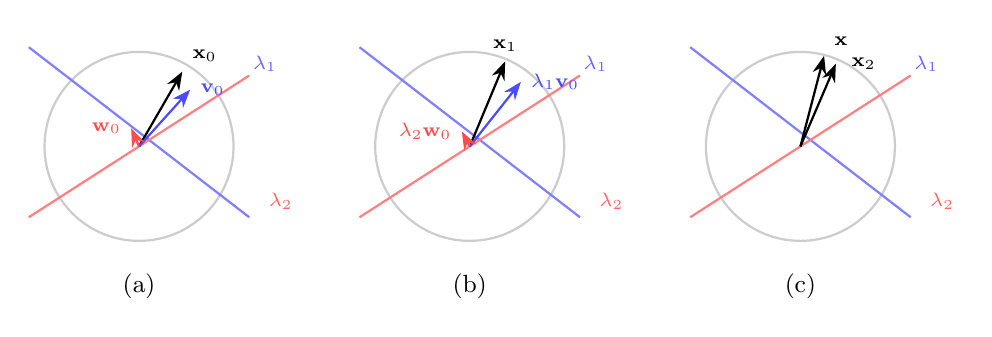
\begin{tikzpicture}[>=Stealth, scale=1.0]
  \foreach \xshift/\lab in {0/(a), 4.2/(b), 8.4/(c)} {
    \draw[thick, gray!40] (\xshift,0) circle (1.2cm);
    \draw[blue!50, thick] (\xshift-1.4,0.9*1.4/1.4*1.4) -- (\xshift+1.4,-0.9);
    \draw[red!50, thick]  (\xshift-1.4,-0.9) -- (\xshift+1.4,0.9);
    \node[font=\scriptsize, blue!60] at (\xshift+1.6,1.05) {$\lambda_1$};
    \node[font=\scriptsize, red!60]  at (\xshift+1.8,-0.7) {$\lambda_2$};
    \node[below, font=\small] at (\xshift,-1.5) {\lab};
  }
  \draw[->, thick, black] (0,0) -- (0.55,0.95) node[above right, font=\scriptsize]{$\mathbf{x}_0$};
  \draw[->, thick, blue!70] (0,0) -- (0.65,0.72) node[right, font=\scriptsize]{$\mathbf{v}_0$};
  \draw[->, thick, red!70]  (0,0) -- (-0.10,0.23) node[left, font=\scriptsize]{$\mathbf{w}_0$};
  \draw[->, thick, black] (4.2,0) -- (4.65,1.08) node[above, font=\scriptsize]{$\mathbf{x}_1$};
  \draw[->, thick, blue!70] (4.2,0) -- (4.85,0.82) node[right, font=\scriptsize]{$\lambda_1\mathbf{v}_0$};
  \draw[->, thick, red!70]  (4.2,0) -- (4.10,0.19) node[left, font=\scriptsize]{$\lambda_2\mathbf{w}_0$};
  \draw[->, thick, black] (8.4,0) -- (8.70,1.15) node[above right, font=\scriptsize]{$\mathbf{x}$};
  \draw[->, thick, black] (8.4,0) -- (8.85,1.05) node[right, font=\scriptsize, xshift=2pt]{$\mathbf{x}_2$};
\end{tikzpicture}
\caption*{FIGURE 9.2.1\quad (a) Initial $\mathbf{x}_0$; (b) after one multiplication;
(c) iterates converge toward eigenspace of $\lambda_1$}
\end{figure}

\vspace{2mm}
\redheading{The Power Method with Euclidean Scaling}

Theorem~9.2.1 gives the following algorithm, called the \textbf{power method with
Euclidean scaling}:

\begin{tcolorbox}[colback=blue!4, colframe=blue!55!black,
  title={\textbf{The Power Method with Euclidean Scaling}},
  boxrule=0.5mm, arc=3mm]
\textbf{Step 0.} Choose an arbitrary nonzero vector; normalize it (if needed) to a unit
vector $\mathbf{x}_0$.

\textbf{Step 1.} Compute $A\mathbf{x}_0$ and normalize to get $\mathbf{x}_1$.
Compute $A\mathbf{x}_1\cdot\mathbf{x}_1$ (first eigenvalue approximation).

\textbf{Step $k$.} Compute $A\mathbf{x}_{k-1}$ and normalize to get $\mathbf{x}_k$.
Compute $A\mathbf{x}_k\cdot\mathbf{x}_k$ ($k$th eigenvalue approximation).

Continuing generates better and better approximations to $\lambda$ and a unit dominant
eigenvector.
\end{tcolorbox}

\subsection*{EXAMPLE 2 | The Power Method with Euclidean Scaling}

Apply the power method with Euclidean scaling to
$A = \begin{bmatrix}3&2\\2&3\end{bmatrix}$, $\mathbf{x}_0=\begin{bmatrix}1\\0\end{bmatrix}$.
Stop at $\mathbf{x}_5$.

\textbf{SOLUTION:} The eigenvalues of $A$ are $\lambda=1$ and $\lambda=5$; the dominant
eigenspace is $x_1=x_2$, with unit dominant eigenvector
$\mathbf{v}_1 = \tfrac{1}{\sqrt{2}}\begin{bmatrix}1\\1\end{bmatrix}
\approx\begin{bmatrix}0.707\ldots\\0.707\ldots\end{bmatrix}$.

\renewcommand{\arraystretch}{1.25}
\begin{center}
\begin{tabular}{|c|l|l|l|}
\hline
$k$ & $A\mathbf{x}_{k-1}$ & $\mathbf{x}_k$ & $\lambda^{(k)} = A\mathbf{x}_k\cdot\mathbf{x}_k$ \\
\hline
1 &
$\begin{bmatrix}3\\2\end{bmatrix}$ &
$\frac{1}{\sqrt{13}}\begin{bmatrix}3\\2\end{bmatrix}\approx\begin{bmatrix}0.83205\\0.55470\end{bmatrix}$ &
$\approx 4.84615$ \\
\hline
2 &
$\approx\begin{bmatrix}3.60555\\3.32820\end{bmatrix}$ &
$\approx\begin{bmatrix}0.73480\\0.67828\end{bmatrix}$ &
$\approx 4.99361$ \\
\hline
3 &
$\approx\begin{bmatrix}3.56097\\3.50445\end{bmatrix}$ &
$\approx\begin{bmatrix}0.71274\\0.70143\end{bmatrix}$ &
$\approx 4.99974$ \\
\hline
4 &
$\approx\begin{bmatrix}3.54108\\3.52976\end{bmatrix}$ &
$\approx\begin{bmatrix}0.70824\\0.70597\end{bmatrix}$ &
$\approx 4.99999$ \\
\hline
5 &
$\approx\begin{bmatrix}3.53666\\3.53440\end{bmatrix}$ &
$\approx\begin{bmatrix}0.70733\\0.70688\end{bmatrix}$ &
$\approx 5.00000$ \\
\hline
\end{tabular}
\end{center}

Thus $\lambda^{(5)}\approx 5.00000$ (five-decimal-place accuracy) and $\mathbf{x}_5$
approximates the dominant unit eigenvector $\mathbf{v}_1$ to three decimal places.

\vspace{2mm}
\redheading{The Power Method with Maximum Entry Scaling}

An alternative normalizes each iterate to make its maximum absolute entry equal to 1.
Denote $\mathrm{max}(\mathbf{x})$ = maximum absolute value of entries of $\mathbf{x}$.

\begin{tcolorbox}[colback=red!4, colframe=red!60!black,
  title={\textbf{Theorem 9.2.2}}, boxrule=0.5mm, arc=3mm]
Let $A$ be a symmetric $n\times n$ matrix with a positive dominant eigenvalue $\lambda$.
If $\mathbf{x}_0$ is a nonzero vector in $R^n$ not orthogonal to the eigenspace of
$\lambda$, then the sequence
\begin{equation}
  \mathbf{x}_0,\quad
  \mathbf{x}_1 = \frac{A\mathbf{x}_0}{\mathrm{max}(A\mathbf{x}_0)},\quad
  \mathbf{x}_2 = \frac{A\mathbf{x}_1}{\mathrm{max}(A\mathbf{x}_1)},\quad\ldots,\quad
  \mathbf{x}_k = \frac{A\mathbf{x}_{k-1}}{\mathrm{max}(A\mathbf{x}_{k-1})},\quad\ldots
  \tag{8}
\end{equation}
converges to an eigenvector corresponding to $\lambda$, and the sequence of
\textbf{Rayleigh quotients}
\begin{equation}
  \frac{A\mathbf{x}_0\cdot\mathbf{x}_0}{\mathbf{x}_0\cdot\mathbf{x}_0},\quad
  \frac{A\mathbf{x}_1\cdot\mathbf{x}_1}{\mathbf{x}_1\cdot\mathbf{x}_1},\quad\ldots,\quad
  \frac{A\mathbf{x}_k\cdot\mathbf{x}_k}{\mathbf{x}_k\cdot\mathbf{x}_k},\quad\ldots
  \tag{9}
\end{equation}
converges to $\lambda$.
\end{tcolorbox}

Each term in (9) is the \textbf{Rayleigh quotient}
\[
  \frac{A\mathbf{x}\cdot\mathbf{x}}{\mathbf{x}\cdot\mathbf{x}} \tag{11}
\]
When $\mathbf{x}$ is a dominant eigenvector, the Rayleigh quotient equals $\lambda$.

\begin{tcolorbox}[colback=blue!4, colframe=blue!55!black,
  title={\textbf{The Power Method with Maximum Entry Scaling}},
  boxrule=0.5mm, arc=3mm]
\textbf{Step 0.} Choose an arbitrary nonzero vector $\mathbf{x}_0$.

\textbf{Step $k$.} Compute $A\mathbf{x}_{k-1}$, scale by $1/\mathrm{max}(A\mathbf{x}_{k-1})$
to get $\mathbf{x}_k$. Compute the Rayleigh quotient of $\mathbf{x}_k$ as the $k$th
eigenvalue approximation.

Continue until convergence.
\end{tcolorbox}

\subsection*{EXAMPLE 3 | Example 2 Revisited Using Maximum Entry Scaling}

Apply the power method with maximum entry scaling to
$A = \begin{bmatrix}3&2\\2&3\end{bmatrix}$, $\mathbf{x}_0=\begin{bmatrix}1\\0\end{bmatrix}$.

\textbf{SOLUTION:}

\renewcommand{\arraystretch}{1.25}
\begin{center}
\begin{tabular}{|c|l|l|l|}
\hline
$k$ & $A\mathbf{x}_{k-1}$ & $\mathbf{x}_k$ &
$\lambda^{(k)} = \dfrac{A\mathbf{x}_k\cdot\mathbf{x}_k}{\mathbf{x}_k\cdot\mathbf{x}_k}$ \\
\hline
1 & $\begin{bmatrix}3\\2\end{bmatrix}$ &
$\frac{1}{3}\begin{bmatrix}3\\2\end{bmatrix}\approx\begin{bmatrix}1.00000\\0.66667\end{bmatrix}$ &
$\approx 4.84615$ \\
\hline
2 & $\approx\begin{bmatrix}4.33333\\4.00000\end{bmatrix}$ &
$\approx\begin{bmatrix}1.00000\\0.92308\end{bmatrix}$ &
$\approx 4.99361$ \\
\hline
3 & $\approx\begin{bmatrix}4.84615\\4.76923\end{bmatrix}$ &
$\approx\begin{bmatrix}1.00000\\0.98413\end{bmatrix}$ &
$\approx 4.99974$ \\
\hline
4 & $\approx\begin{bmatrix}4.96825\\4.95238\end{bmatrix}$ &
$\approx\begin{bmatrix}1.00000\\0.99681\end{bmatrix}$ &
$\approx 4.99999$ \\
\hline
5 & $\approx\begin{bmatrix}4.99361\\4.99042\end{bmatrix}$ &
$\approx\begin{bmatrix}1.00000\\0.99936\end{bmatrix}$ &
$\approx 5.00000$ \\
\hline
\end{tabular}
\end{center}

The Rayleigh quotients $\lambda^{(k)}$ agree with those from Euclidean scaling.
Maximum entry scaling produces an eigenvector approaching $\begin{bmatrix}1\\1\end{bmatrix}$
(set $t=1$ in the parametric form~(6)).

\vspace{2mm}
\redheading{Rate of Convergence}

If $|\lambda_1|>|\lambda_2|\geq|\lambda_3|\geq\cdots\geq|\lambda_k|$, the rate at which
Rayleigh quotients converge to $\lambda_1$ depends on the ratio $|\lambda_1|/|\lambda_2|$.
The larger the ratio, the faster the convergence. In Example~3, $|\lambda_1|/|\lambda_2|=5/1=5$,
which is why convergence is rapid.

\vspace{2mm}
\redheading{Stopping Procedures}

If $\lambda$ is the exact dominant eigenvalue and $\lambda^{(k)}$ is the $k$th
approximation, the \textbf{relative error} in $\lambda^{(k)}$ is $|\lambda-\lambda^{(k)}|/|\lambda|$.
In practice, $\lambda$ is unknown, so we use the \textbf{estimated relative error}:
\begin{equation}
  \left|\frac{\lambda^{(k)}-\lambda^{(k-1)}}{\lambda^{(k)}}\right| < E \tag{13}
\end{equation}
to stop the iteration when accuracy $E$ is achieved.

\subsection*{EXAMPLE 4 | Estimated Relative Error}

For the computations in Example~3, find the smallest $k$ for which the estimated
percentage error in $\lambda^{(k)}$ is less than~$0.1\%$.

\textbf{SOLUTION:}

\renewcommand{\arraystretch}{1.3}
\begin{center}
\begin{tabular}{|c|l|l|}
\hline
$\lambda^{(k)}$ &
$\left|\dfrac{\lambda^{(k)}-\lambda^{(k-1)}}{\lambda^{(k)}}\right|$ &
Estimated \% error \\
\hline
$\lambda^{(2)}\approx4.99361$ &
$\left|\dfrac{4.99361-4.84615}{4.99361}\right|\approx0.02953$ & $2.953\%$ \\
\hline
$\lambda^{(3)}\approx4.99974$ &
$\approx0.00123$ & $0.123\%$ \\
\hline
$\lambda^{(4)}\approx4.99999$ &
$\approx0.00005$ & $0.005\%$ \\
\hline
$\lambda^{(5)}\approx5.00000$ &
$\approx0.00000$ & $0.000\%$ \\
\hline
\end{tabular}
\end{center}

Thus $\lambda^{(4)}=4.99999$ is the first approximation with estimated percentage error
below~$0.1\%$.

\vspace{3mm}
\noindent\rule{\linewidth}{0.5pt}

\section*{Exercise Set 9.2}

\noindent\textit{In Exercises 1--2, distinct eigenvalues are given. Determine whether $A$
has a dominant eigenvalue, and if so, find it.}

\begin{enumerate}
  \item \textbf{a.} $\lambda_1=7,\ \lambda_2=3,\ \lambda_3=-8,\ \lambda_4=1$\quad
        \textbf{b.} $\lambda_1=-5,\ \lambda_2=3,\ \lambda_3=2,\ \lambda_4=5$

  \item \textbf{a.} $\lambda_1=1,\ \lambda_2=0,\ \lambda_3=-3,\ \lambda_4=2$\quad
        \textbf{b.} $\lambda_1=-3,\ \lambda_2=-2,\ \lambda_3=-1,\ \lambda_4=3$

\end{enumerate}

\noindent\textit{In Exercises 3--4, apply the power method with Euclidean scaling to $A$,
starting with $\mathbf{x}_0$, stopping at $\mathbf{x}_4$.}

\begin{enumerate}
  \item[3.] $A = \begin{bmatrix}5&-1\\-1&-1\end{bmatrix}$;\quad
        $\mathbf{x}_0 = \begin{bmatrix}1\\0\end{bmatrix}$

  \item[4.] $A = \begin{bmatrix}7&-2&0\\-2&6&-2\\0&-2&5\end{bmatrix}$;\quad
        $\mathbf{x}_0 = \begin{bmatrix}1\\0\\0\end{bmatrix}$

\end{enumerate}

\noindent\textit{In Exercises 5--6, apply the power method with maximum entry scaling to
$A$, starting with $\mathbf{x}_0$, stopping at $\mathbf{x}_4$.}

\begin{enumerate}
  \item[5.] $A = \begin{bmatrix}1&-3\\-3&5\end{bmatrix}$;\quad
        $\mathbf{x}_0 = \begin{bmatrix}1\\1\end{bmatrix}$

  \item[6.] $A = \begin{bmatrix}3&2&2\\2&2&0\\2&0&4\end{bmatrix}$;\quad
        $\mathbf{x}_0 = \begin{bmatrix}1\\1\\1\end{bmatrix}$

\end{enumerate}

\begin{enumerate}
  \item[7.] Let $A = \begin{bmatrix}2&-1\\-1&2\end{bmatrix}$,
        $\mathbf{x}_0=\begin{bmatrix}1\\0\end{bmatrix}$.

  \textbf{a.} Apply the power method with maximum entry scaling; round to 3 decimal places;
  stop after 3 iterations.

  \textbf{b.} Use the result in (a) and the Rayleigh quotient to approximate the dominant
  eigenvalue.

  \textbf{c.} Find the exact dominant eigenvector and eigenvalue.

  \textbf{d.} Find the percentage error in the eigenvalue approximation from (b).

\end{enumerate}

\noindent\textit{In Exercises 9--10, a matrix $A$ with a dominant eigenvalue and a power
sequence $\mathbf{x}_0, A\mathbf{x}_0,\ldots,A^5\mathbf{x}_0$ are given. Use
Formulas~(9) and (10) to approximate the dominant eigenvalue and a corresponding
eigenvector.}

\begin{enumerate}
  \item[9.] $A = \begin{bmatrix}1&2\\2&1\end{bmatrix}$;\quad
        $\mathbf{x}_0=\begin{bmatrix}1\\0\end{bmatrix}$,\;
        $A\mathbf{x}_0=\begin{bmatrix}1\\2\end{bmatrix}$,\;
        $A^2\mathbf{x}_0=\begin{bmatrix}5\\4\end{bmatrix}$,\;
        $A^3\mathbf{x}_0=\begin{bmatrix}13\\14\end{bmatrix}$,\;
        $A^4\mathbf{x}_0=\begin{bmatrix}41\\40\end{bmatrix}$,\;
        $A^5\mathbf{x}_0=\begin{bmatrix}121\\122\end{bmatrix}$

\end{enumerate}

\begin{enumerate}
  \item[11.] Consider $A = \begin{bmatrix}-1&0\\0&0\end{bmatrix}$ and
        $\mathbf{x}_0 = \begin{bmatrix}a\\b\end{bmatrix}$ (a unit vector, $a\ne 0$).
        Show that even though $A$ is symmetric and has a dominant eigenvalue, the
        power sequence~(1) in Theorem~9.2.1 does not converge. This shows that the
        requirement that the dominant eigenvalue be positive is essential.

  \item[12.] Use the power method with Euclidean scaling to approximate the dominant
        eigenvalue and a corresponding eigenvector of $A$; stop when the estimated
        percentage error in the eigenvalue approximation is less than $0.1\%$.

        \textbf{a.} $A = \begin{bmatrix}1&3&3\\3&4&-1\\3&-1&10\end{bmatrix}$

  \item[15.] Prove: If $A$ is a nonzero $n\times n$ matrix, then $A^TA$ and $AA^T$ have
        positive dominant eigenvalues.

\end{enumerate}

\end{document}
